% !Mode:: "TeX:UTF-8"
% !TEX program  = xelatex
\documentclass{sdureport}
% no head line or foot line
%\pagestyle{empty}

% just for filling a few pages
\usepackage{blindtext}
\usepackage{ctex}
\usepackage{indentfirst}
\usepackage{amsmath}
\usepackage{upgreek}
\usepackage{listings}
\usepackage{anyfontsize} % 公式字体报错问题
\usepackage{float}%提供float浮动环境
\usepackage{booktabs}%提供命令\toprule、\midrule、\bottomrule
\usepackage{multirow}%提供跨列命令\multicolumn{}{}{}
\usepackage{graphicx}
\usepackage{subfigure}
\usepackage{epstopdf}

% initialize the variable texts
\sduCollege{网络空间安全}
\sduCourse{网络安全创新创业实践}
\sduName{张涵/彭炜霖/李庭跃}
\sduExperimentalTopics{任务1：比特币测试网交易发送与底层数据解析}
\sduExexperimentalHours{4h}
\sduDate{2026年7月20日}

\begin{document}
\begin{sduDocument}
	\section{实验目的：}
	\begin{enumerate}
		\renewcommand{\labelenumi}{(\theenumi)}
		\item 掌握比特币测试网的基本交互操作，包括轻节点钱包的配置、测试币水龙头的使用及交易发送。
		\item 通过编写 Python 数据解析脚本，亲自动手复现并验证工作量证明(PoW)机制中的双重 SHA-256 哈希计算过程。
	\end{enumerate}
	
	\section{实验步骤：}
	\subsection{实验环境：}
	\subsubsection{软件环境：}
	\begin{itemize}
		\item Electrum 4.8.0 轻量级钱包 (Testnet 模式)
		\item mempool.space 比特币测试网区块链浏览器
		\item Python 3
	\end{itemize}
	\subsubsection{硬件环境：}
	\begin{itemize}
		\item 个人计算机 (Ubuntu 虚拟机终端环境)
	\end{itemize}

	\subsection{实验内容}
	本次实验要求完成从链上交互到本地数据逆向解析的完整闭环，主要包含以下内容：
	\begin{enumerate}
		\renewcommand{\labelenumi}{(\theenumi)}
		\item \textbf{网络交互与交易上链}：在 Linux 终端下载并运行 Electrum 钱包，申请测试币并对外发送一笔转账。
		\item \textbf{原始数据获取}：利用 Mempool 浏览器查询所发交易的 TXID，分别提取出该笔交易的完整 Raw Hex，以及包含该交易的区块其标准的 80 字节区块头原始十六进制数据。
		\item \textbf{逐字节数据解析}：根据区块链协议规范，编写解析脚本。最终实现对输入输出金额、脚本长度及锁定时间的精准拆解，并成功验证 PoW 工作量哈希。
	\end{enumerate} 

	\section{代码实现：}
	\subsection{Python解析脚本 (task1.py)}
	为了兼容隔离见证交易，并严格校验区块头长度以防数据抓取错误，本实验设计了如下解析代码：
	\begin{lstlisting}[language=python]
import hashlib

def little_endian_to_int(hex_str):
    #将小端序十六进制字符串转换为整数
    return int.from_bytes(bytes.fromhex(hex_str), byteorder='little')

def double_sha256(hex_string):
    #计算双重SHA256
    first_hash = hashlib.sha256(bytes.fromhex(hex_string)).digest()
    second_hash = hashlib.sha256(first_hash).digest()
    return second_hash[::-1].hex()

def parse_block_header(header_hex):

    print("      解析 Block Header       ")
    header_hex = header_hex.strip()

    version = header_hex[0:8]
    prev_hash = header_hex[8:72]
    merkle_root = header_hex[72:136]
    timestamp = header_hex[136:144]
    bits = header_hex[144:152]
    nonce = header_hex[152:160]

    print(f"1. Version (版本号): {version} -> {little_endian_to_int(version)}")
    print(f"2. Previous Block Hash: \n   {prev_hash}")
    print(f"3. Merkle Root: \n   {merkle_root}")
    print(f"4. Timestamp (时间戳): {timestamp} -> {little_endian_to_int(timestamp)}")
    print(f"5. Difficulty Target (Bits): {bits}")
    print(f"6. Nonce (随机数): {nonce} -> {little_endian_to_int(nonce)}")

    calculated_hash = double_sha256(header_hex)
    print(f"\n[PoW 验证] 计算本区块头的双重 SHA256 哈希:\n{calculated_hash}")

def parse_transaction(raw_tx):
    print("      解析 Transaction      ")

    raw_tx = raw_tx.strip()
    cursor = 8
    version = raw_tx[:8]
    print(f"Version: {version} -> {little_endian_to_int(version)}")

    if raw_tx[cursor:cursor + 4] == "0001":
        cursor += 4

    in_count_hex = raw_tx[cursor:cursor + 2]
    in_count = little_endian_to_int(in_count_hex)
    print(f"\nInput Count (输入数量): {in_count_hex} -> {in_count}")
    cursor += 2

    for i in range(in_count):
        print(f"\n--- [Input {i}] ---")
        txid_hex = raw_tx[cursor:cursor + 64]
        print(f"Previous TX Hash: \n  {bytes.fromhex(txid_hex)[::-1].hex()}")
        cursor += 64

        vout = raw_tx[cursor:cursor + 8]
        print(f"Previous Output Index: {vout} -> {little_endian_to_int(vout)}")
        cursor += 8

        script_sig_len = little_endian_to_int(raw_tx[cursor:cursor + 2])
        cursor += 2
        print(f"Unlocking Script Length: {script_sig_len} 字节")

        if script_sig_len > 0:
            script_sig = raw_tx[cursor:cursor + (script_sig_len * 2)]
            print(f"Unlocking Script: {script_sig}")
            cursor += (script_sig_len * 2)
        else:
            print(f"Unlocking Script: 空 ")

        sequence = raw_tx[cursor:cursor + 8]
        print(f"Sequence Number: {sequence}")
        cursor += 8

    out_count_hex = raw_tx[cursor:cursor + 2]
    out_count = little_endian_to_int(out_count_hex)
    print(f"\nOutput Count (输出数量): {out_count_hex} -> {out_count}")
    cursor += 2

    for i in range(out_count):
        print(f"\n--- [Output {i}] ---")
        amount = raw_tx[cursor:cursor + 16]
        satoshi = little_endian_to_int(amount)
        print(f"Amount (聪/Satoshi): {amount} -> {satoshi} ({satoshi / 1e8} tBTC)")
        cursor += 16

        script_pubkey_len = little_endian_to_int(raw_tx[cursor:cursor + 2])
        cursor += 2
        print(f"Locking Script Length: {script_pubkey_len} 字节")

        script_pubkey = raw_tx[cursor:cursor + (script_pubkey_len * 2)]
        print(f"Locking Script: \n  {script_pubkey}")
        cursor += (script_pubkey_len * 2)

    locktime = raw_tx[-8:]
    print(f"\nLocktime (锁定时间): {locktime} -> {little_endian_to_int(locktime)}")


tx_hex = (
    "02000000000101bfa57dc098d76c993f66084b5bcbefd25f"
	"d185f65cf07f2fa2edf58dd3cdff5f0000000000fdffffff"
    "021027000000000000160014c8c43f9b09e2aadeb3fc1d20"
	"0da042443bfd3b90a47d0100000000001600148720f7d193"
    "ac7dacf3ccee15d44a5a1b970aac290247304402203b2be4"
	"07b36e2e30da0e4910d59ba4fca11773762a470a3d9726f0"
    "ce43470426022016f44f3b79a993556657d31f3bd15e2cad"
	"3bb56699e6579e6dc82652b4aecb47012102fbc4a496077b"
    "6a3368989f25e72e60b77270b36642689dbca75f731a693f"
	"4b1d00000000"
)

header_hex = (
    "04000020aa40636186cdd62d715c429ca2d7e3b7b09056f7"
	"00f5f72dec254b3300000000c80a53071babea49096231d0"
	"76ce91fc8509f15c99b56dc6f7de05e0feb794118adb5d6a"
	"ffff001d59f13a5f"
)

if __name__ == "__main__":
    parse_block_header(header_hex)
    parse_transaction(tx_hex)
	\end{lstlisting} 

	\section{结果输出分析：}
	\subsection{终端执行结果}
	通过执行 `task1.py` 脚本，针对抓取到的测试网数据进行解析，控制台成功输出了符合逻辑的区块结构与交易明细：
	\begin{lstlisting}[language=bash]
      解析 Block Header       
1. Version (版本号): 04000020 -> 536870916
2. Previous Block Hash: 
   aa40636186cdd62d715c429ca2d7e3b7b09056f700f5f72dec254b3300000000
3. Merkle Root: 
   c80a53071babea49096231d076ce91fc8509f15c99b56dc6f7de05e0feb79411
4. Timestamp (时间戳): 8adb5d6a -> 1784535946
5. Difficulty Target (Bits): ffff001d
6. Nonce (随机数): 59f13a5f -> 1597698393

[PoW 验证] 计算本区块头的双重 SHA256 哈希:
000000001f28dc7c06309babbc26e9f461a58fc8f4f072b9835366b58fcae6af
      解析 Transaction      
Version: 02000000 -> 2

Input Count (输入数量): 01 -> 1

--- [Input 0] ---
Previous TX Hash: 
  5fffcdd38df5eda22f7ff05cf685d15fd2efcb5b4b08663f996cd798c07da5bf
Previous Output Index: 00000000 -> 0
Unlocking Script Length: 0 字节
Unlocking Script: 空 
Sequence Number: fdffffff

Output Count (输出数量): 02 -> 2

--- [Output 0] ---
Amount (聪/Satoshi): 1027000000000000 -> 10000 (0.0001 tBTC)
Locking Script Length: 22 字节
Locking Script: 
  0014c8c43f9b09e2aadeb3fc1d200da042443bfd3b90

--- [Output 1] ---
Amount (聪/Satoshi): a47d010000000000 -> 97700 (0.000977 tBTC)
Locking Script Length: 22 字节
Locking Script: 
  00148720f7d193ac7dacf3ccee15d44a5a1b970aac29

Locktime (锁定时间): 00000000 -> 0
	\end{lstlisting}

	测试结果截图如下：
	\begin{figure}[H]
		\centering
		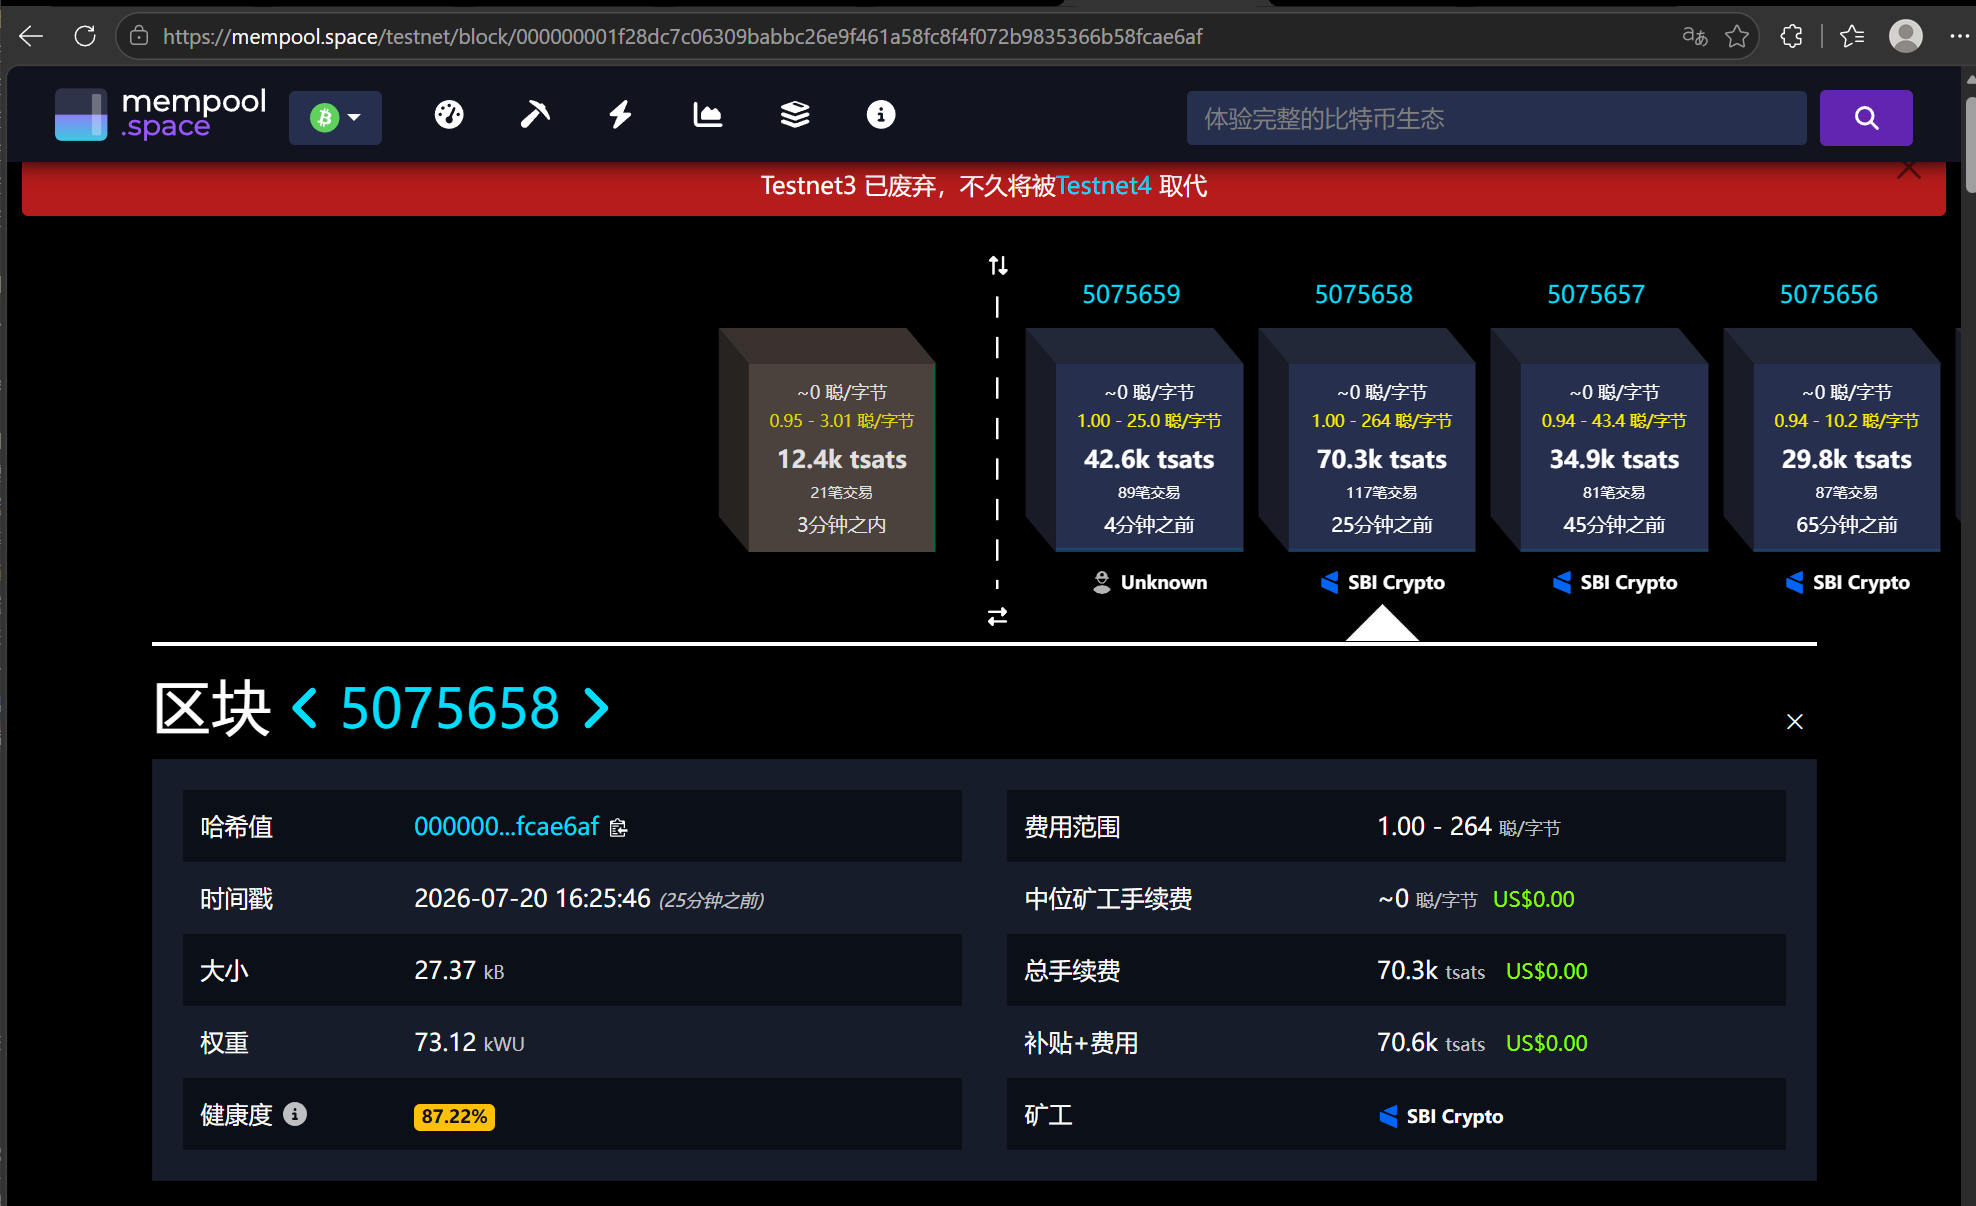
\includegraphics[width=0.9\textwidth]{result.png}
		\caption{实验结果截图}
	\end{figure}

\end{sduDocument}
\end{document}